\documentclass[border=10pt]{standalone}
\usepackage{tikz}
\usetikzlibrary{positioning, shapes.geometric, calc}

\tikzset{
  box/.style={
    rectangle, rounded corners, draw=black, thick, align=center, inner xsep=6pt, inner ysep=4pt, font=\small
  },
  line/.style={draw=black, thick}
}

\begin{document}
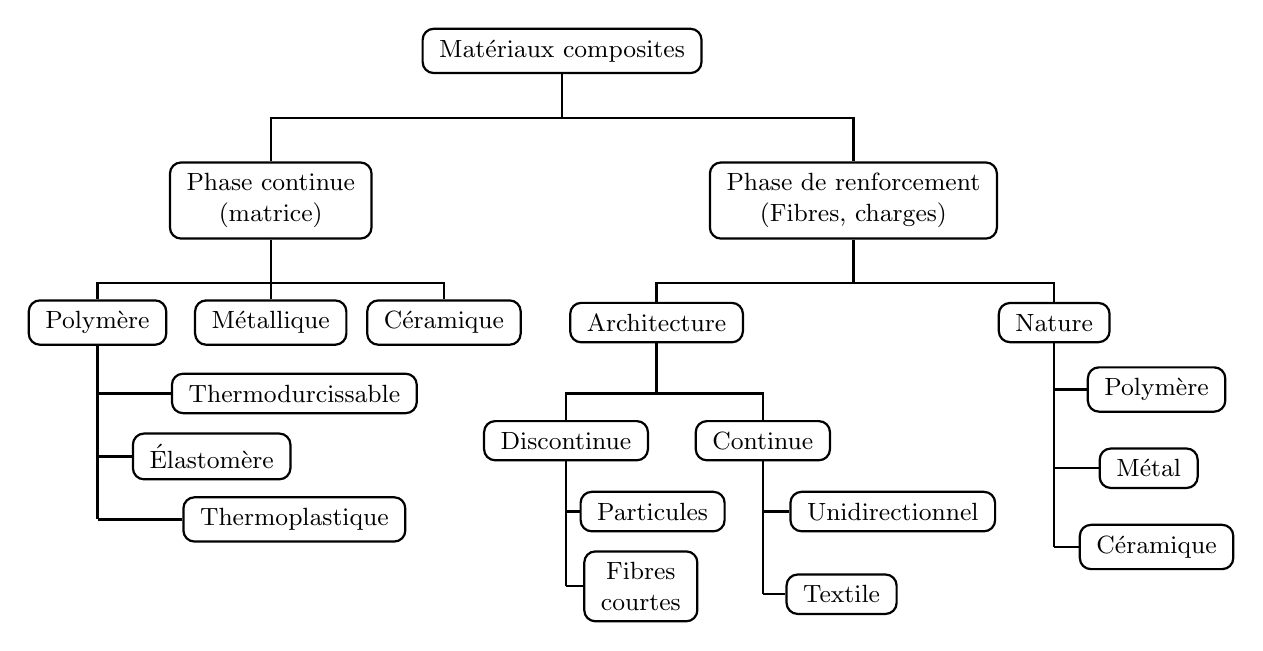
\begin{tikzpicture}

% Root node
\node[box] (root) at (0,0) {Matériaux composites};

% First level
\node[box] (phase_continue) at (-3.7,-1.9) {Phase continue\\(matrice)};
\node[box] (phase_renforcement) at (3.7,-1.9) {Phase de renforcement\\(Fibres, charges)};

% Connect root to first level
\coordinate (topbranch) at (0,-0.85);
\draw[line] (root.south) -- (topbranch);
\draw[line] (topbranch) -- (-3.7,-0.85) -- (phase_continue.north);
\draw[line] (topbranch) -- (3.7,-0.85) -- (phase_renforcement.north);

% Phase continue branch
\node[box] (polymere) at (-5.9,-3.45) {Polymère};
\node[box] (metal) at (-3.7,-3.45) {Métallique};
\node[box] (ceramique) at (-1.5,-3.45) {Céramique};

\coordinate (pcbranch) at (-3.7,-2.95);
\draw[line] (phase_continue.south) -- (pcbranch);
\draw[line] (pcbranch) -- (-5.9,-2.95) -- (polymere.north);
\draw[line] (pcbranch) -- (metal.north);
\draw[line] (pcbranch) -- (-1.5,-2.95) -- (ceramique.north);

% Polymere subtypes
\node[box] (thermodurcissable) at (-3.4,-4.35) {Thermodurcissable};
\node[box] (elastomere) at (-4.45,-5.15) {Élastomère};
\node[box] (thermoplastique) at (-3.4,-5.95) {Thermoplastique};

\draw[line] (polymere.south) -- (polymere.south |- thermoplastique.west);
\draw[line] (polymere.south |- thermodurcissable.west) -- (thermodurcissable.west);
\draw[line] (polymere.south |- elastomere.west) -- (elastomere.west);
\draw[line] (polymere.south |- thermoplastique.west) -- (thermoplastique.west);

% Phase reinforcement branch
\node[box] (architecture) at (1.2,-3.45) {Architecture};
\node[box] (nature) at (6.25,-3.45) {Nature};

\coordinate (prbranch) at (3.7,-2.95);
\draw[line] (phase_renforcement.south) -- (prbranch);
\draw[line] (prbranch) -- (1.2,-2.95) -- (architecture.north);
\draw[line] (prbranch) -- (6.25,-2.95) -- (nature.north);

% Architecture subtypes
\node[box] (discontinue) at (0.05,-4.95) {Discontinue};
\node[box] (continue) at (2.55,-4.95) {Continue};

\coordinate (archbranch) at (1.2,-4.35);
\draw[line] (architecture.south) -- (archbranch);
\draw[line] (archbranch) -- (0.05,-4.35) -- (discontinue.north);
\draw[line] (archbranch) -- (2.55,-4.35) -- (continue.north);

% Discontinue subtypes
\node[box] (particules) at (1.15,-5.85) {Particules};
\node[box] (fibres_courtes) at (1.00,-6.80) {Fibres\\courtes};

\draw[line] (discontinue.south) -- (discontinue.south |- fibres_courtes.west);
\draw[line] (discontinue.south |- particules.west) -- (particules.west);
\draw[line] (discontinue.south |- fibres_courtes.west) -- (fibres_courtes.west);

% Continue subtypes
\node[box] (unidirectionnel) at (4.20,-5.85) {Unidirectionnel};
\node[box] (textile) at (3.55,-6.90) {Textile};

\draw[line] (continue.south) -- (continue.south |- textile.west);
\draw[line] (continue.south |- unidirectionnel.west) -- (unidirectionnel.west);
\draw[line] (continue.south |- textile.west) -- (textile.west);

% Nature subtypes
\node[box] (polymere_nature) at (7.55,-4.30) {Polymère};
\node[box] (metal_nature) at (7.45,-5.30) {Métal};
\node[box] (ceramique_nature) at (7.55,-6.30) {Céramique};

\draw[line] (nature.south) -- (nature.south |- ceramique_nature.west);
\draw[line] (nature.south |- polymere_nature.west) -- (polymere_nature.west);
\draw[line] (nature.south |- metal_nature.west) -- (metal_nature.west);
\draw[line] (nature.south |- ceramique_nature.west) -- (ceramique_nature.west);

\end{tikzpicture}
\end{document}
